%--------------------------------------------------------------------------------------------------------------------------------%
% Code and text for "Understanding how population structure affects pathogen richness in a mechanistic model of bat populations"
% Chapter 3 of thesis "The role of population structure and size in determining bat pathogen richness"
% by Tim CD Lucas
%
% NB The file is numbered Chapter2 as this was previously Chapter 2 in the thesis.
%
%---------------------------------------------------------------------------------------------------------------------------------%











\section{Abstract}


\tmpsection{One or two sentences providing a basic introduction to the field}
% comprehensible to a scientist in any discipline.
\lettr{A}n increasingly large proportion of emerging human diseases comes from animals.
These diseases have a huge impact on human health, healthcare systems and economic development.
The chance that a new zoonosis will come from any particular wild host species increases with the number of pathogen species occurring in that host species.
However, the factors that control pathogen richness of wild animal species remain unclear.
%
%
\tmpsection{Two to three sentences of more detailed background}
% comprehensible to scientists in related disciplines.
% Add mechanistic vs empirical
Comparative, phylogenetic studies have shown that host-species traits such as population density, longevity and body size correlate with pathogen richness.
Further comparative studies have found correlations between population structure and pathogen richness.
Typically it is assumed that well-connected, unstructured populations (that therefore have a high basic reproductive number, $R_0$) promote the invasion of new pathogens and therefore increase pathogen richness. % Where or how to define well-connected?
However, this assumption is largely untested.
In the presence of inter-pathogen competition, the opposite effect might occur; increased population structure may increase pathogen richness by reducing the effects of competition.
A more mechanistic understanding of how population structure affects pathogen richness could discriminate between these two broad hypotheses.
%
\tmpsection{One sentence clearly stating the general problem (the gap)}
% being addressed by this particular study.
%It is unknown whether greater population structure allows invading pathogens to escape from competition by stochastically creating areas of low pathogen prevalence.
I hypothesised that both low dispersal rates and a low number of connections in a metapopulation network would allow invading pathogens to establish more easily, thus increasing pathogen richness. 
I tested these hypotheses using metapopulation networks parameterised to mimic wild bat populations as bats have highly varied social structures and have recently been implicated in a number of high profile diseases such as Ebola, SARS, Hendra and Nipah.
%
%
\tmpsection{One sentence summarising the main result}
%  (with the words “here we show” or their equivalent).
I simulated the process of a new pathogen invading into a metapopulation already occupied by an identical pathogen.
I varied the dispersal rate, topology of the metapopulation and transmission rate.
I found significant evidence that increased dispersal rate increased the probability that a new pathogen would invade into a population.
I found marginal evidence that network topology affected the probability that a new pathogen would invade.
%\paragraph{Two or three sentences explaining what the main result reveals in direct comparison to what was thought to be the case previously}
% or how the main result adds to previous knowledge
The assumption that factors causing high $R_0$ allow new pathogens to invade and therefore increase pathogen richness was supported.
However, my results contradict many theoretical studies which predict that increased population structure should promote coexistence of pathogens.
My results also contradict empirical patterns of pathogen richness with respect to population structure.
Therefore, it is likely that population structure affects pathogen richness via a different mechanism to the one modelled here.
%
%
\tmpsection{One or two sentences to put the results into a more general context.}


%\tmpsection{Two or three sentences to provide a broader perspective, }
% readily comprehensible to a scientist in any discipline.





%%%%%%%%%%%%%%%%%%%%%%%%%%%%%%%%%%%%%%%%%%%%%%%%%%%%%%%%%%%%%%%%%%%%%%%%%%%%%%%%%%%%%%%%%%%%%%%%%%%%%%%%%%%%%%%%%%%%%%%%%%%%%%%%%%%%%%%%%%%%%%%%%%%%%%%%%%%


\section{Introduction}

%%%%%%%%%%%%%%%%%%%%%%%%%%%%%%%%%%%%%%%%%%%%%%%%%%%%%%%%%%%%%%%%%%%%%%%%%%%%%%%%%%%%%%%%%%%%%%%%%%%%%%%%%%%%%%%%%%%%%%%%%%%%%%%%%%%%%%%%%%%%%%%%%%%%%%%%%%%


%Possible structure (each number a sep. paragraph):
%1. zoonotics bad, need to predict spillover, factors controlling pathogen richness unknown
%2. results from comparative studies (including mammal and bat ones), explaining why population structure is important
%3. limitations of comparative studies (including highlighting that empirical and mechanistic approaches would give different predictions) that and need a more mechanistic approach 
%4. description of the possible mechanisms for population structure - explaining why focusing on reduction of competition mechanisms
%5. results from analytical models so far and limitations of the approach
%6. what is needed now
%7. what your focus is (including a  bit about bat focus)
%8. 'here I show..' what you found briefly to lead into methods




\tmpsection{General Intro}
%%%%%%%%%%%%%%%%%%%%%%%%%%%%%%
% A basic introduction to the field,
% comprehensible to a scientist in any discipline.

%1. zoonotics bad, need to predict spillover, factors controlling pathogen richness unknown
\tmpsection{Why is pathogen richness? important?}
Over 50\% of emerging infectious diseases have an animal source \cite{jones2008global, smith2014global}.
Zoonotic pathogens can be highly virulent \cite{luby2009recurrent, lefebvre2014case} and can have huge public health impacts \cite{granich2015trends}, economic costs \cite{knobler2004learning} and slow down international development \cite{ebolaWorldbank}.
Therefore understanding and predicting changes in the process of zoonotic spillover is a global health priority \cite{taylor2001risk}.
The number of pathogen species hosted by a wild animal species affects the chance that a disease from that species will infect humans \cite{wolfe2000deforestation}.
However, the factors that control the number of pathogen species in a wild animal population are still unclear \cite{metcalf2015five}; in particular our mechanistic understanding of how population processes inhibit or promote pathogen richness is poor.



\tmpsection{Specific Intro}
%%%%%%%%%%%%%%%%%%%%%%%%%%%%%%
% more detailed background}
% comprehensible to scientists in related disciplines.


\tmpsection{We know some factors that correlate with pathogen richness}
%population density, longevity, body size and population structure

%2. results from comparative studies (including mammal and bat ones), explaining why population structure is important
%3. limitations of comparative studies (including highlighting that empirical and mechanistic approaches would give different predictions) that and need a more mechanistic approach 

In comparative studies, a number of host traits have been shown to correlate with pathogen richness including body size \cite{kamiya2014determines, arneberg2002host}, population density \cite{nunn2003comparative, arneberg2002host} and range size \cite{bordes2011impact, kamiya2014determines}.
A further factor that may affect pathogen richness is population structure.
In comparative studies it is often assumed that factors that promote fast disease spread should promote high pathogen richness; the faster a new pathogen spreads through a population, the more likely it is to persist \cite{nunn2003comparative, morand2000wormy, poulin2014parasite, poulin2000diversity, altizer2003social}.
However, this assumption ignores competitive mechanisms such as cross-immunity and depletion of susceptible hosts.
If competitive mechanisms are strong, endemic pathogens in populations structured such that $R_0$ will be high will be able to easily out-compete invading pathogens.
%Only if competitive mechanisms are weak will high $R_0$  enable the invasion of new pathogens and allow higher pathogen richness.

Overall, the evidence from comparative studies indicates that increased population structure correlates with higher pathogen richness.
This conclusion is based on studies using a number of measures of population structure: genetic measures, the number of subspecies, the shape of species distributions and social group size (Chapter \ref{ch:empirical}, \cites{vitone2004body, maganga2014bat, turmelle2009correlates}).
However, there are a number of studies that contradict this conclusion \cite{gay2014parasite, bordes2007rodent, ezenwa2006host}.
Comparative studies are often contradictory due to small sample sizes, noisy data and because empirical relationships often do not extrapolate well to other taxa. 
Furthermore, multicollinearity between many traits also makes it hard to clearly distinguish which factors are important \cite{nunn2015infectious}.
However, meta-analyses can be used to combine studies to help generalise conclusions \cite{kamiya2014determines}.


%3. limitations of comparative studies (including highlighting that empirical and mechanistic approaches would give different predictions) that and need a more mechanistic approach 

Furthermore, knowing which factors correlate with pathogen richness does not tell us if, or how, they causally control pathogen richness.
This lack of a solid mechanistic understanding of these processes prevents predictions of how wild populations will respond to perturbations such as increased human pressure and global change.
As habitats fragment we expect wild populations to change in a number of ways including becoming smaller and less well connected \cite{andren1994effects, cushman2012separating}.
As multiple population-level factors are likely to change simultaneously due to global change, the correlative relationships examined in comparative studies are unlikely to effectively predict future changes in pathogen richness.
Mechanistic models are needed to project how these highly non-linear disease systems will respond to the multiple, simultaneous stressors affecting them.



\tmpsection{Network structure has been studied}
%5. results from analytical models so far and limitations of the approach
%4. description of the possible mechanisms for population structure - explaining why focusing on reduction of competition mechanisms

There are a number of mechanisms by which population structure could increase pathogen richness.
Firstly, population structure may reduce competition between pathogens.
In analytical models of well-mixed populations competitive exclusion has been predicted \cite{ackleh2003competitive, bremermann1989competitive, martcheva2013competitive, qiu2013vector, allen2004sis}.
In models where competitive exclusion occurs in well-mixed populations, population structure has sometimes been shown to allow coexistence \cite{qiu2013vector, allen2004sis, nunes2006localized, garmer2016multistrain}.
Alternatively, population structure may promote the evolution of new strains within a species \cite{buckee2004effects}, reduce the rate of pathogen extinction \cite{rand1995invasion} or increase the probability of pathogen invasion from other host species \cite{nunes2006localized}.
These separate mechanisms have not been examined and it is difficult to see how they could be distinguished through comparative methods.

%Competing epidemics, or two pathogens spreading at the same time in a population, is a well studied area \cite{poletto2013host, poletto2015characterising, karrer2011competing}. 
%This area is related to the study of pathogen richness in that they indicate that dynamics of multiple pathogens in a population do depend on population %structure.
%However, the results for short term epidemic competition do not directly transfer to the study of long term disease persistence.


%6. what is needed now
\tmpsection{The gap}
%%%%%%%%%%%%%%%%%%%%%%%%%%%%%%
% One sentence clearly stating the general problem
% being addressed by this particular study.
% By this stage, must have defined/introduced all terms used within.

Currently, the literature contains very abstract, simplified models \cite{qiu2013vector, allen2004sis, garmer2016multistrain, may1994superinfection}.
These cannot be easily applied to real data.
They also do not easily give quantitative predictions of pathogen richness; typically they predict either no pathogen coexistence \cite{bremermann1989competitive, martcheva2013competitive} or infinite pathogen richness \cite{may1994superinfection}.
Models that can give quantitive predictions of pathogen richness in wild populations are more applicable to real-world issues such as zoonotic disease surveillance.
While predicting an absolute value of pathogen richness for a wild species is likely to be impossible, models that attempt to rank species from highest to lowest pathogen richness are still useful for prioritising species for surveillance.
This requires a middle ground of model complexity.

\tmpsection{What I did}
%%%%%%%%%%%%%%%%%%%%%%%%%%%%%%
%7. what your focus is (including a  bit about bat focus)

In order to capture this middle ground, I have used metapopulation models. 
Unlike two-patch models that are used to add population structure while keeping model complexity to a minumum \cite{qiu2013vector, allen2004sis, garmer2016multistrain}, the metapopulations used here split the population into multiple subpopulations.
I have used two independant variables that alter population structure: dispersal rate and metapopulation network topology.
I have studied the invasion of new pathogens as a mechanism for increasing pathogen richness.
In particular I have focused on studying the invasion of a newly evolved pathogen that is therefore identical in epidemiological parameters to the endemic pathogen.
Furthermore, this close evolutionary relationship means that competition via cross-immunity is strong.

\tmpsection{Why bats}
The metapopulations were parameterised to broadly mimic wild bat populations.
Population structure has already been found to correlate with pathogen richness in bats (Chapter \ref{ch:empirical}, \cites{gay2014parasite, maganga2014bat, turmelle2009correlates}).
Furthermore, bats have an unusually large variety of social structures.
Colony sizes range from ten to 1 million individuals \cite{jones2009pantheria} and colonies can be very stable \cite{kerth2011bats, mccracken1981social}.
This strong colony fidelity means they fit the assumptions of metapopulations well.
Bats have also, over the last decade, become a focus for disease research \cite{calisher2006bats, hughes2007emerging}.
The reason for this focus is that they have been implicated in a number of high profile diseases including Ebola, SARS, Hendra and Nipah \cite{calisher2006bats, li2005bats}.

%8. 'here I show..' what you found briefly to lead into methods

\tmpsection{What I found}
%%%%%%%%%%%%%%%%%%%%%%%%%%%%%%
% One sentence summarising the main result
% (with the words “here we show” or their equivalent).

Here I show that, given the assumptions of a metapopulation, increased dispersal significantly increased the probability of invasion of new pathogens.
Furthermore, structured populations nearly always had a lower probability of pathogen invasion than fully-mixed populations of equal size.
The topology of the network did not strongly affect the probability of pathogen invasion as long as the population was not completely unconnected.
Overall, I found significant evidence that reduced population structure increases the probability of invasion of a new pathogen, implying a role for the generation of pathogen richness more generally.


%%%%%%%%%%%%%%%%%%%%%%%%%%%%%%%%%%%%%%%%%%%%%%%%%%%%%%%%%%%%%%%%%%%%%%%%%%%%%%%%%%%%%%%%%%%%%%%%%%%%%%%%%%%%%%%%%%%%%%%%%%%%%%%%%%%%%%%%%%%%%%%%%%%%%%%%%%%

\section{Methods}

%%%%%%%%%%%%%%%%%%%%%%%%%%%%%%%%%%%%%%%%%%%%%%%%%%%%%%%%%%%%%%%%%%%%%%%%%%%%%%%%%%%%%%%%%%%%%%%%%%%%%%%%%%%%%%%%%%%%%%%%%%%%%%%%%%%%%%%%%%%%%%%%%%%%%%%%%%%

%%


\subsection{Two pathogen SIR model}

I developed a multipathogen, SIR compartment model with individuals being classed as susceptible, infected or recovered with immunity (Figure~\ref{f:sir}).
Susceptible individuals are counted in class $S$ (see Table~\ref{t:params} for a list of symbols and values used).
There are three infected classes, $I_1$, $I_2$ and $I_{12}$, being individuals infected with Pathogen 1, Pathogen 2 or both respectively.
Recovered individuals, $R$, are immune to both pathogens, even if they have only been infected with one (i.e.\ there is complete cross-immunity).
Furthermore, recovery from one pathogen moves an individual straight into the recovered class, even if the individual is infected with both pathogens (Figure~\ref{f:sir}).
This modelling choice allows the model to be easily expanded to include more than two pathogens, though this study is restricted to two pathogens.
The assumption of immediate recovery from all other diseases is likely to be reasonable.
Any up-regulation of innate immune response will affect both pathogens equally.
Furthermore, as the pathogens are identical, any acquired immunity would also affect both pathogens equally.

The coinfection rate (the rate at which an infected individual is infected with a second pathogen) is adjusted compared to the infection rate by a factor $\alpha$.
Low values of $\alpha$ imply lower rates of coinfection.
In particular, $\alpha = 0$ indicates no coinfections, $\alpha = 1$ indicates that coinfections happen at the same rate as first infections while $\alpha > 1$ indicates that coinfections occur more readily than first infections.


In the application of long term existence of pathogens it is necessary to include vital dynamics (births and deaths) as the SIR model without vital dynamics has no endemic state.
Birth and death rates ($\mu$ and $\Lambda$) are set as being equal meaning the population does not systematically increase or decrease.
The population size does however change as a random walk.
New born individuals enter the susceptible class.
Infection amd coinfection were assumed to cause no extra mortality as for a number of viruses, bats show no clinical signs of infection \cite{halpin2011pteropid, deThoisy2016bioecological}.
%In humans, coinfection generally worsens health \cite{griffiths2011nature} but as there are 

\tmpsection{Metapopulation}


The population is modelled as a metapopulation, being divided into a number of subpopulations (colonies).
This model is an intermediate level of complexity between fully-mixed populations and contact networks.
The existence of subspecies, measurements of genetic dissimilarity and ecological studies provide ample evidence that bat populations are structured to some extent \cite{kerth2011bats, mccracken1981social, burns2014correlates, wilson2005mammal}.
Therefore a fully mixed population is a large oversimplification.
However, trying to study the contact network relies on knowledge of detailed individual behaviour which is rarely available.		

The metapopulation is modelled as a network with colonies being nodes and dispersal between colonies being indicated by edges (Figure~\ref{f:net}).
Individuals within a colony interact randomly so that the colony is fully mixed.
Dispersal between colonies occurs at a rate $\xi$.
Individuals can only disperse to colonies connected to theirs by an edge in the network.
The rate of dispersal is not affected by the number of edges a colonies has (known as the degree of the colony and denoted $k$).
Therefore, the dispersal rate from a colony $x$ with degree $k_x$ to colony $y$ is $\xi / k_x$.
Note this rate is independent of the degree and size of colony $y$.



\tmpsection{Stochastic simulations}

I examined this model using stochastic, continuous-time simulations implemented in \emph{R} \cite{R}.
The implementation is available as an \emph{R} package on GitHub \cite{metapopepi}.
The model can be written as a continuous-time Markov chain.
The Markov chain contains the random variables $((S_x)_{x = 1\ldots m}, (I_{x, q})_{x =1\ldots m,\:q \in \{1, 2, 12\}}, (R_x)_{x = 1\ldots m})$.
Here, $(S_x)_{x = 1\ldots m}$ is a length $m$ vector of the number of susceptibles in each colony.
$(I_{x, q})_{x =1\ldots m, q \in \{1, 2, 12\}}$ is a length $m \times 3$ vector describing the number of individuals of each disease class ($q \in \{1, 2, 12\}$) in each colony.
Finally, $(R_x)_{x = 1\ldots m}$ is a length $m$ vector of the number of individuals in the recovered class.
The model is a Markov chain where extinction of both pathogens species and extinction of the host species are absorbing states.
However, the expected time to reach this state is much larger than the duration of the simulations.

At any time, suppose the system is in state $((s_x), (i_{x,q}), (r_x))$.
At each step in the simulation we calculate the rate at which each possible event might occur.
One event is then randomly chosen, weighted by its rate
\begin{align}
  p(\text{event } i) = \frac{e_i}{\sum_j e_j},
\end{align}
where $e_i$ is the rate at which event $i$ occurs and $\sum_j e_j$ is the sum of the rates of all possible events.
Finally, the length of the time step, $\delta$, is drawn from an exponential distribution 
\begin{align}
  \delta \sim \operatorname{Exp}\left(\sum_i e_i  \right).
\end{align}


\begin{figure}[t]
\centering
  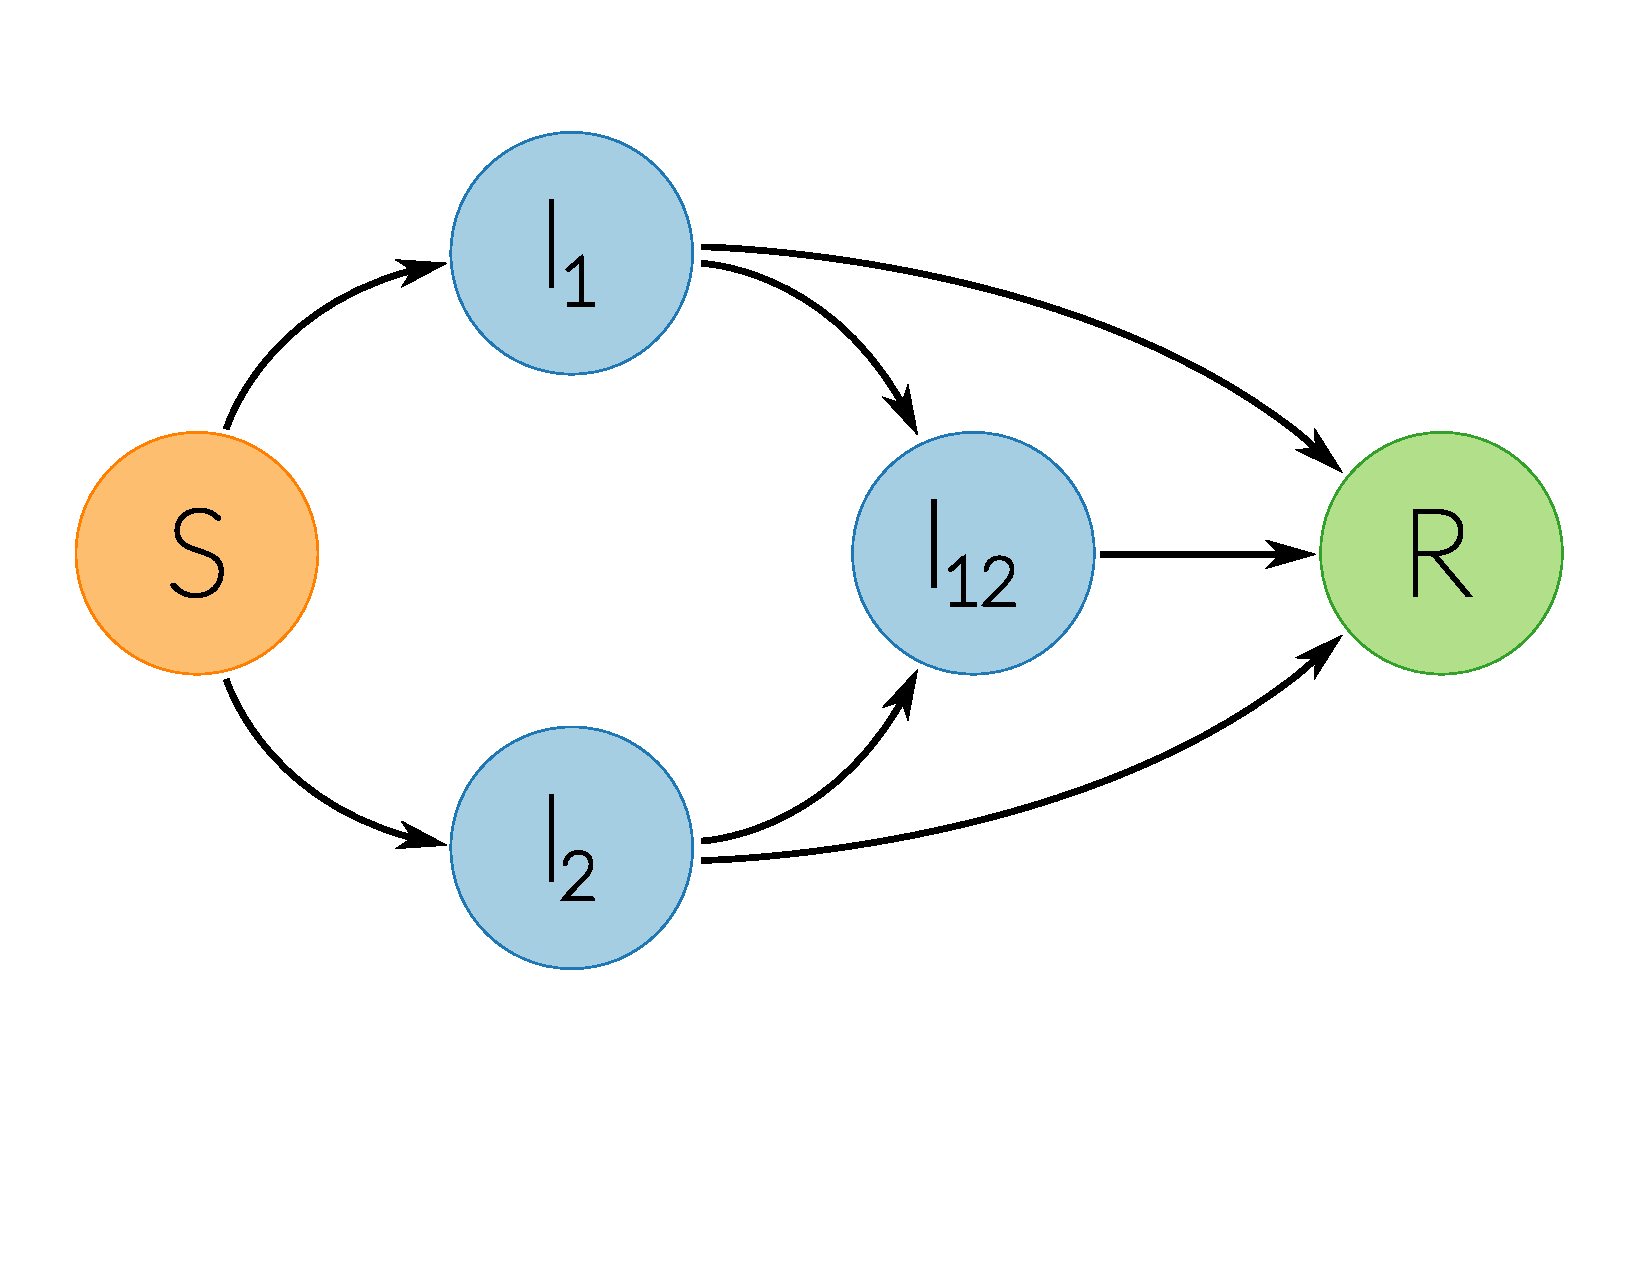
\includegraphics[width=0.5\textwidth]{imgs/SIRoption1.pdf}
  \caption[Schematic of the SIR model used]{
  Schematic of the SIR model used. 
  Individuals are in one of five classes, susceptible (orange, $S$), infected with Pathogen 1, Pathogen 2 or both (blue, $I_1, I_2, I_{12}$) or recovered and immune from further infection (green, $R$).
  Transitions between epidemiological classes occur as indicated by solid arrows.
  Vital dynamics (births and deaths) are indicated by dashed arrows.
  Parameter symbols for transitions are indicated.
  Note that individuals in $I_{12}$ move into $R$, not back to $I_1$ or $I_2$. 
  That is, recovery from one pathogen causes immediate recovery from the other pathogen.
  }
\label{f:sir}
\end{figure}


We can now write down the rates of all events. 
%I defined $I^+_p$ to be the sum of all classes that are infectious with pathogen $p$, for example $I^+_1 = I_1 + I_{12}$. 
Assuming asexual reproduction, that all classes reproduce at the same rate and that individuals are born into the susceptible class we get
\begin{align}
  s_x \rightarrow s_x + 1 \;\;\text{at a rate of}\;\; \Lambda\left( s_{x}+\sum_q i_{qx} + r_{x}\right) 
\end{align}
where $s_x \rightarrow s_x + 1$ is the event that the number of susceptibles in colony $x$ will increase by 1 (a single birth) and $\sum_q i_{qx}$ is the sum of all infection classes $q \in \{1, 2, 12\}$.
The rates of death, given a death rate $\mu$, and no increased mortality due to infection, are given by
\begin{align}
  s_x \rightarrow s_x-1  &\;\;\text{at a rate of}\;\; \mu s_x, \\
  i_{qx}  \rightarrow i_{qx}-1 &\;\;\text{at a rate of}\;\; \mu i_{qx},\\
  r_x  \rightarrow r_x-1 &\;\;\text{at a rate of}\;\; \mu r_x.
\end{align}


\begin{table}[b!]
\centering
\caption[All symbols used in Chapters \ref{ch:sims1} and \ref{ch:sims2}.]{A summary of all symbols used in Chapters \ref{ch:sims1} and \ref{ch:sims2} along with their units and default values.
The justification for parameter values is given in Section \ref{s:paramSelect}.}

\begin{tabular}{@{}lp{6cm}p{2.9cm}r@{}}
\toprule
Symbol & Explanation & Units & Value\\
\midrule
$\rho$ & Number of pathogens && 2\\
$x, y$ & Colony index &&\\
$p$ &  Pathogen index i.e.\ $p\in\{1,2\}$ for pathogens 1 and 2 & &\\
$q$ & Disease class i.e.\ $q\in\{1,2,12\}$&\\
$S_x$ & Number of susceptible individuals in colony $x$ &&\\
$I_qx$ & Number of individuals infected with disease(s) $q \in {1, 2, 12}$ in colony $x$ &&\\
$R_x$ & Number of individuals in colony $x$ in the recovered with immunity class  &&\\
$N$ & Total Population size && 30,000\\
$m$ & Number of colonies&& 10\\
$n$ & Colony size && 3,000\\
$a$ & Area & \si{\square\kilo\metre}& 10,000\\
$\beta$ & Transmission rate &  & 0.1 -- 0.4\\
$\alpha$ & Coinfection adjustment factor.  & Proportion & 0.1\\
$\gamma$ & Recovery rate & year$^{-1}.$individual$^{-1}$ & 1\\
$\xi$ & Dispersal & year$^{-1}.$individual$^{-1}$ & 0.001--0.1\\
$\Lambda$ & Birth rate & year$^{-1}.$individual$^{-1}$ & 0.05\\
$\mu$ & Death rate & year$^{-1}.$individual$^{-1}$ & 0.05\\
$k_x$ & Degree of node $x$ (number of colonies that individuals from colony $x$ can disperse to). &&\\
$\delta$ & Waiting time until next event & years &\\

$e_i$ & The rate at which event $i$ occurs & year$^{-1}$&\\
\bottomrule
\end{tabular}

\label{t:params}
\end{table}


I modelled transmission as being density-dependent.
This assumption was more suitable than frequency-dependent transmission as I was modelling a disease transmitted by saliva or urine in highly dense populations confined to caves, buildings or potentially a small number of tree roosts.
I was notably not modelling a sexually transmitted disease (STD) as spillover of STDs from bats to humans is likely to be rare.
Infection of a susceptible with either Pathogen 1 or 2 is therefore given by
\begin{align}
  i_{1x} \rightarrow i_{1x}+1, s_x \rightarrow s_x-1 &\;\;\text{at a rate of}\;\; \beta s_x\left(i_{1x} + i_{12x}\right),\\
  i_{2x} \rightarrow i_{2x}+1, s_x \rightarrow s_x-1  &\;\;\text{at a rate of}\;\; \beta s_x\left(i_{2x} + i_{12x}\right),
\end{align}
while coinfection, given the coinfection adjustment factor $\alpha$, is given by
\begin{align}
  i_{12,x} \rightarrow i_{12,x}+1,\: i_{1x} \rightarrow i_{1x}-1 &\;\;\text{at a rate of}\;\; \alpha\beta i_{1x}\left(i_{2x} + i_{12x}\right),\\
  i_{12,x} \rightarrow i_{12,x}+1,\: I_{2x} \rightarrow i_{2x}-1 &\;\;\text{at a rate of}\;\; \alpha\beta i_{2x}\left(i_{1x} + i_{12x}\right).
\end{align}
Note that lower values of $\alpha$ give lower rates of infection as in \textcite{castillo1989epidemiological}.


The probability of migration from colony $y$ (with degree $k_y$) to colony $x$, given a dispersal rate $\xi$ is given by
\begin{align}
  s_x \rightarrow s_x+1,\: s_y \rightarrow s_y-1 &\;\;\text{at a rate of}\;\; \frac{\xi s_y}{k_y},\\
  i_{qx} \rightarrow i_{qx}+1,\: i_{qy} \rightarrow i_{qy}-1 &\;\;\text{at a rate of}\;\; \frac{\xi i_{qy}}{k_y},\\
  r_x \rightarrow r_x+1,\: r_y \rightarrow r_y-1 &\;\;\text{at a rate of}\;\; \frac{\xi r_y}{k_y}.
\end{align}
Not that the dispersal rate does not change with infection.
As above, this is due to the low virulence of bat viruses.
Finally, recovery from any infectious class occurs at a rate $\gamma$
\begin{align}
  i_{qx} \rightarrow i_{qx}-1,\: r_x \rightarrow r_x+1  \;\;\text{at a rate of}\;\; \gamma i_{qx}.
\end{align}


\begin{figure}[t]
{\centering 
\subfloat[Fully connected\label{fig:fullyConnected}]{
  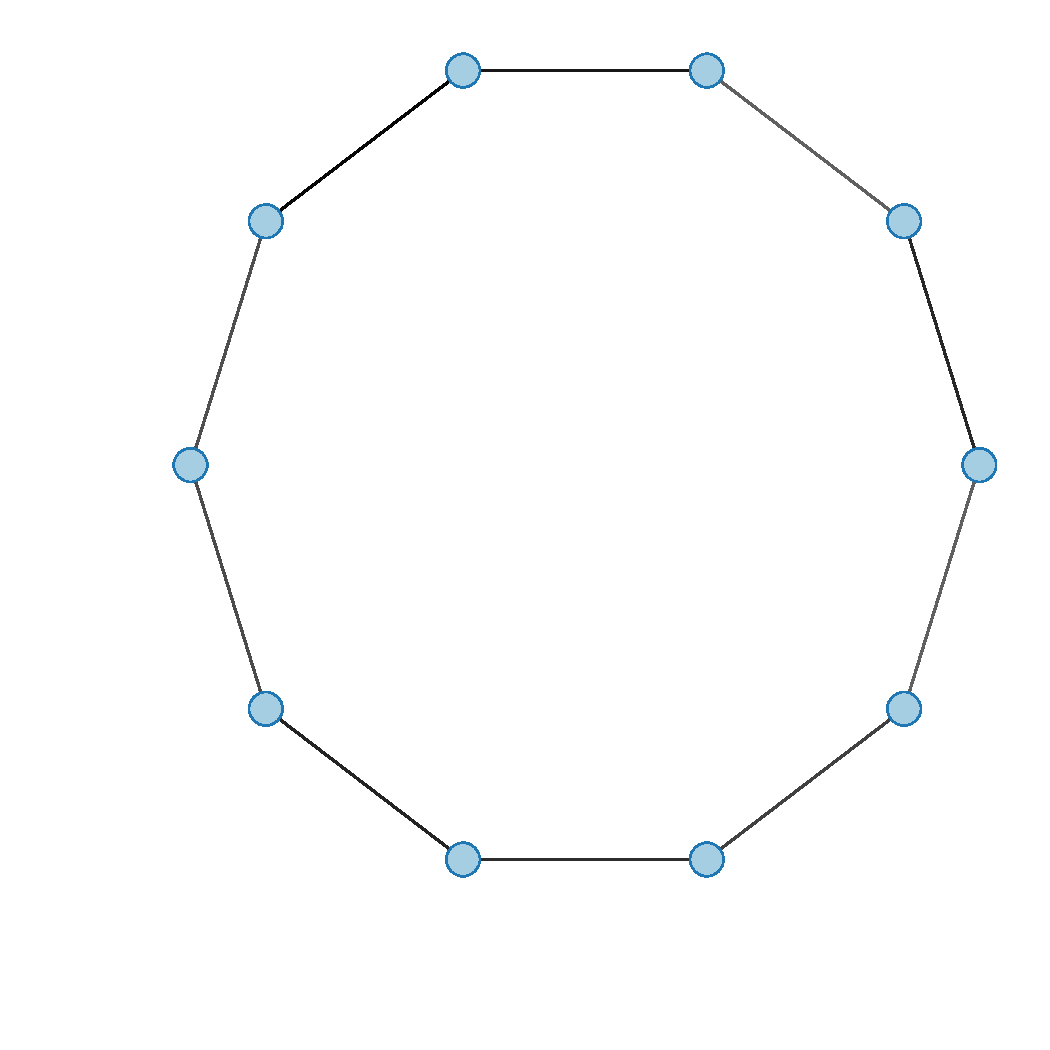
\includegraphics[width=0.45\textwidth]{imgs/minimallyConnected.pdf} 
}
\subfloat[Minimally connected
\label{fig:minimallyConnected}]{
  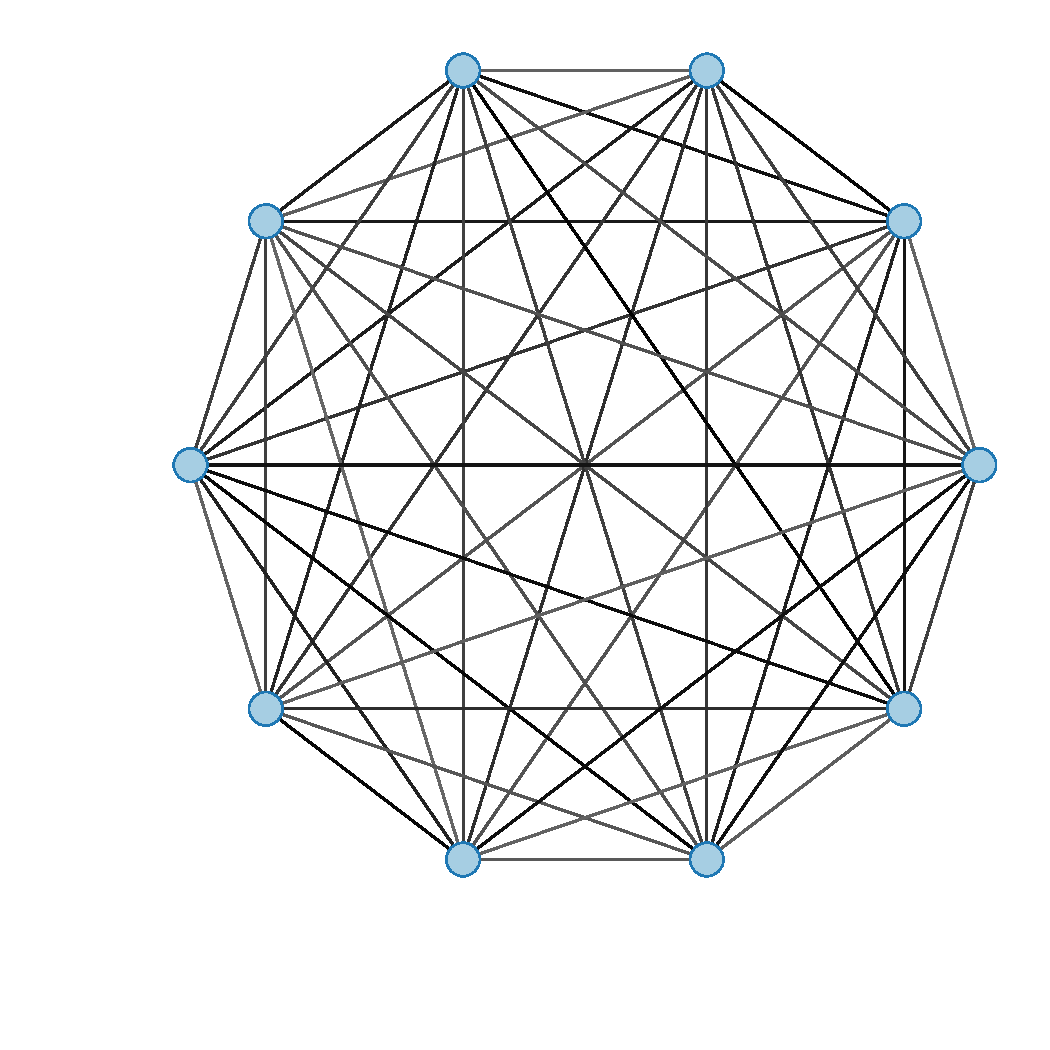
\includegraphics[width=0.45\textwidth]{imgs/fullyConnected.pdf} 
}
}
\caption[Network topologies used to compare network connectedness]{
The two network topologies used to test whether network connectedness influences a pathogen's ability to invade.
A) Animals can only disperse to neighbouring colonies. 
B) Dispersal can occur between any colony.
Blue circles are colonies of \SI{3000} individuals.
Dispersal only occurs between colonies connected by an edge (black line).
The dispersal rate is held constant between the two topologies.
}
\label{f:net}
\end{figure}








% ------------------------------------------------------------------ %
% Dispersal Sims
% ------------------------------------------------------------------ %















% ------------------------------------------------------------------ %
% Topology Sims
% ------------------------------------------------------------------ %












% ------------------------------------------------------------------ %
% Unstructured Sims
% ------------------------------------------------------------------ %















\subsection{Parameter selection}
\label{s:paramSelect}

The fixed parameters were chosen to roughly reflect realistic wild bat populations. 
The death rate $\mu$ was set as 0.05 per year giving a generation time of 20 years.
The birth rate $\Lambda$ was set to be equal to $\mu$.
This yields a population that does not systematically increase or decrease.
However, the size of each colony changes as a random walk.
Given the length of the simulations, colonies were very unlikely to go extinct (Figure~\ref{fig:plotsNoInvade2}).
The starting size of each colony was set to \SI{3000}. 
This is appropriate for many bat species \cite{jones2009pantheria}, especially the large, frugivorous \emph{Pteropodidae} that have been particularly associated with recent zoonotic diseases.

The recovery rate $\gamma$ was set to one, giving an average infection duration of one year. 
This is therefore a long lasting infection but not a chronic infection. 
It is very difficult to directly estimate infection durations in wild populations but it seems that these infections might sometimes be long lasting \cite{peel2012henipavirus, plowright2015ecological}.
However, other studies have found much shorter infectious periods \cite{amengual2007temporal}.
These shorter infections are not studied further here. %todo consider readding this. " as preliminary simulations found that they could not persist in the relatively small populations being modelled here."

Four values of the transmission rate $\beta$ were used, 0.1, 0.2, 0.3 and 0.4.
These values were chosen to cover the range of behaviours, from very high probabilities of invasion of the second pathogen, to very low probabilities.
All simulations were run under all four transmission rates as this is such a fundamental parameter.
The coinfection adjustment parameter, $\alpha$, was set to 0.1 so that an individual infected with one pathogen is 90\% less likely to be infected with another.
This is a rather arbitrary value.
However, the rationale of the model was that the invading species might be a newly speciated strain of the endemic species.
Furthermore, the model assumes complete cross-immunity after recovery from infection.
Therefore cross-immunity to coinfection is likely to be very strong as well.
Some pairs of closely related bat viruses have been found to coinfect individual bats less than would be expected by chance \cite{anthony2013strategy}.
This indicates a level of cross-immunity between these pairs of viruses. %todo I'm sure there was a marburg ebola paper...





\subsection{Experimental setup}

The metapopulation was made up of ten colonies.
Ten colonies was selected as a trade-off between computation time and a network complex enough that any effects of population structure could be detected.
This value is artificially small compared to wildlife populations. 
In each simulation, the na{\"i}ve population was seeded with ten sets of 200 infected individuals of Pathogen 1.
These groups were seeded into randomly selected colonies with replacement.
For each 200 infected individuals added, 200 susceptible individuals were removed to keep starting colony sizes constant. 
Pathogen 1 was then allowed to spread until the initial, large epidemic had ended. 
Visual inspection of preliminary simulations was used to decide on \SI{300000} events as being long enough for the epidemic to end and the pathogen to be in an endemic state (Figures~\ref{fig:plotsInvade} and \ref{fig:plotsNoInvade1}).
After \SI{300000} events, five individuals infected with Pathogen 2 were added to one randomly selected colony. 
After another \SI{500000} events the invasion of Pathogen 2 was considered successful if any individuals were still infected with Pathogen 2.
Therefore, if at least one individual was in class $I_2$ or $I_{12}$ at the end of the simulation, this was considered an invasion.
Again, visual inspection of preliminary simulations was used to determine that after \SI{500000} events, if an invading pathogen was still present, it was well established (Figures~\ref{fig:plotsInvade} and \ref{fig:plotsNoInvade1}).

The choice to use a fixed number of events, rather than a fixed number of years, was for computational convenience.
However, this choice creates a risk of bias as simulations with more events per unit time will last for a shorter time overall.
However, visual inspection of the dynamics of disease extinction (\ref{fig:plotsNoInvade1}), and examination of the typical time to extinction implies that this bias is very weak.
For example, of the simulations where extinction occurred, the extinction occurred more than 50 years before the end of the simulation in 90\% of cases.
On a preliminary run of 106 simulations across all combinations of dispersal and transmission rates, examining the population after \SI{700000} events instead of \SI{800000} events gave exactly the same result with respect to the binary state of invasion or no invasion. 


\subsection{Population structure}

As a baseline for comparison, I ran simulations of a fully unstructured population.
These simulations were run with a population of \SI{30000} so that the total population size was equal to that of the total metapopulation size in the structured simulations.
I ran 100 simulations at each transmission rate.


\tmpsection{Dispersal}
%%%%%%%%%%%%%%%%%%%%%%%%%%%%%%


Two parameters control population structure in the model: dispersal rate and the topology of the metapopulation network.
The values used for these parameters were chosen to highlight the effects of population structure. 
I selected the dispersal rates $\xi = 0, 0.1, 0.01$ and $ 0.001$ dispersals per individual per year. 
The probability that an individual disperses at least once in its lifetime is given by $\xi / \left(\xi + \mu\right)$.
Therefore, $\xi = 0.1$ relates to 67\% of individuals dispersing between colonies at least once in their lifetime. 
Exclusively juvenile dispersal would have dispersal rates similar to this value. %todo cite
$\xi = 0.01$ relates to 17\% of individuals dispersing at least once in their lifetime.
This value is relatively close to male-biased dispersal, with female philopatry. %todo cite
This therefore relates to a species that does not habitually disperse.
Finally, I ran simulations with no dispersal.
Given zero dispersal, only the colony seeded with Pathogen 2 could ever recieve infections of the invading pathogen.
Therefore, only one colony was simulated for $\xi = 0$.
I ran 100 simulations for most parameter sets.
I ran 150 simulations for $\xi = 0.1, 0.01$ and $0.001$ with $\beta = 0.2$ and $0.3$ as
Preliminary simulations indicated that any effects of population structure would most likely be seen at these values so extra simulations were run to increase statistical power. 



\tmpsection{Network structure}
%%%%%%%%%%%%%%%%%%%%%%%%%%%%%%
I also altered the topology of the metapopulation network.
The network topology was created to be either fully or minimally connected (Figure~\ref{f:net}). 
To model a completely unconnected population the $\xi = 0$ simulations from above were used.
I again ran 100 simulations for each parameter set.



\subsection{Statistical analysis}

I used generalised linear models (GLMs) with a binary response variable, invasion or not, to test the hypothesis that probability of invasion increased with dispersal.
Seperate GLMs were fitted for each transmission rate.
These tests were performed both with and without the $\xi = 0$ results as the complete lack of dispersal makes these simulations qualitatively different to the other simulations.
To test whether the different topologies had different probabilities of invasion, I used Fisher's exact tests because topology is best described as a categorical variable.
As with the $\xi = 0$ results, these tests were performed both with and without the completely unconnected topology results.
Finally, I also used binomial GLMs to test the hypothesis that the probability of invasion increased with transmission rate.
Seperate GLMs were fitted for each dispersal rate and network topology.
All statistical analyses were performed using the \emph{stats} package in \emph{R}.
The code used for running the simulations and analysing the results is available at \url{https://github.com/timcdlucas/PhDThesis/blob/master/Chapter2.Rtex}.


%%%%%%%%%%%%%%%%%%%%%%%%%%%%%%%%%%%%%%%%%%%%%%%%%%%%%%%%%%%%%%%%%%%%%%%%%%%%%%%%%%%%%%%%%%%%%%%%%%%%%%%%%%%%%%%%%%%%%%%%%%%%%%%%%%%%%%%%%%%%%%%%%%%%%%%%%%%


\section{Results}

%%%%%%%%%%%%%%%%%%%%%%%%%%%%%%%%%%%%%%%%%%%%%%%%%%%%%%%%%%%%%%%%%%%%%%%%%%%%%%%%%%%%%%%%%%%%%%%%%%%%%%%%%%%%%%%%%%%%%%%%%%%%%%%%%%%%%%%%%%%%%%%%%%%%%%%%%%%











































\begin{knitrout}\footnotesize
\definecolor{shadecolor}{rgb}{0.969, 0.969, 0.969}\color{fgcolor}\begin{figure}[t]

{\centering 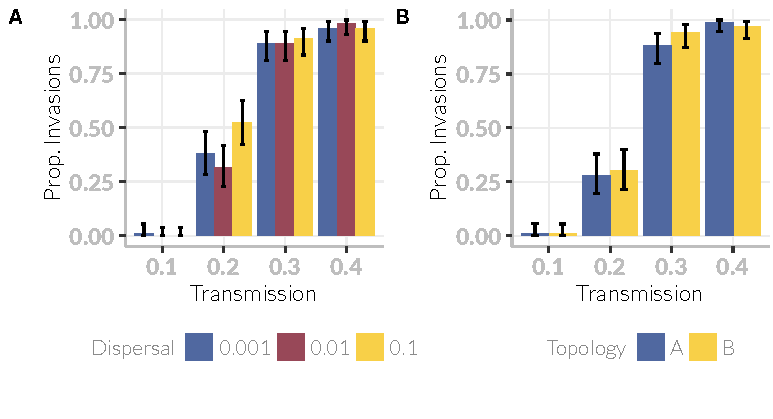
\includegraphics[width=\textwidth]{figure/invasionPropPlots-1} 

}

\caption[The probability of invasion across different dispersal rates and network topologies.]{
  The probability of successful invasion for different A) dispersal rates and B) network topologies (with network topologies ``unconnected'', ``minimally connected'' and ``fully connected'' as in Figure~\ref{f:net}). 
  Error bars are 95\% confidence intervals of probability of invasion. 
  100 simulations were run for each treatment except $\beta = 0.2$ in A) which has 150 per treatment.
  Other parameters were kept constant at: $m = 10,\, \, \mu = \Lambda = 0.05,\, \gamma = 1,\, \alpha = 0.1$. 
  When dispersal is varied, the population structure is fully connected. 
  When network topology is varied, $\xi = 0.01$.}\label{f:invasionPropPlots}
\end{figure}


\end{knitrout}


\subsection{Dispersal}
%%%%%%%%%%%%%%%%%%%%%%%%%%%%%%

In the unstructured population, the second pathogen invaded in 100 out of 100 simulations.
This was true at all four transmission rates.

When the $\xi = 0$ simulations were included, there was a positive relationship between dispersal rate and invasion probability for $\beta = 0.2, 0.3$ and $0.4$ (Figure~\ref{f:invasionPropPlots}A, Table~\ref{B-disp}).
These positive relationships were all significant (GLM. $\beta = 0.2$: $b$ = 12.59, $p < 10^{-5}$. $\beta = 0.3$: $b$ = 12.07, $p$ = 0. $\beta = 0.4$: $b$ = 13.44, $p$ = 0.03.)
At $\beta = 0.1$ there was no significant relationship as invasion probaiblity was very close to zero at all dispersal rates (GLM. $b$ = \ensuremath{-220.19}, $p$ = 0.62).

However, when the $\xi = 0$ simulations were removed, this significant, positive relationship largely disappeared.
At $\beta = 0.2$, the significant positive relationship remained (GLM: $b$ = 7.97, $p$ = 0).
At all other transmission rates, the probability of invasion did not significantly change with dispersal rate (GLM. $\beta = 0.1$: $b$ = \ensuremath{-1928.77}, $p$ = 1. $\beta = 0.3$: $b$ = 0.27, $p$ = 0.94. $\beta = 0.4$: $b$ = \ensuremath{-2.7}, $p$ = 0.70.)


\subsection{Network topology}
%%%%%%%%%%%%%%%%%%%%%%%%%%%%%%

When the completely unconnected topology simulations were included, the probability of invasion was different across topologies for $\beta = 0.2, 0.3$ and $0.4$ (Fisher's exact test. $\beta = 0.2$:  $p < 10^{-5}$. $\beta = 0.3$: $p < 10^{-5}$. $\beta = 0.4$:  $p < 10^{-5}$).
In each case, the fully unconnected population had a lower probability of invasion than the minimally and completely connected topologies (Figure~\ref{f:invasionPropPlots}B, Table~\ref{B-topo}).
At $\beta = 0.1$ there was no significant difference ($p = 0.77$) and the probability of invasion was close to zero for all topologies (Figure~\ref{f:invasionPropPlots}B).

When the completely unconnected topology simulations were removed, there were no significant differences between topologies i.e.\ between the minimally and fully connected topologies (Figure~\ref{f:invasionPropPlots}B). 
This was true at all transmission rates (Fisher's exact test. $\beta = 0.1$, $p = 1.00$. $\beta = 0.2$,  $p = 0.88$. $\beta = 0.3$, $p = 0.22$. $\beta = 0.4$,  $p = 0.62$).



\subsection{Transmission}
%%%%%%%%%%%%%%%%%%%%%%%%%%

Increasing the transmission rate increased the probability of invasion (Figure~\ref{f:invasionPropPlots}).
This was true for all four dispersal values (GLM. $\xi = 0$: $b$ = 19.73, $p < 10^{-5}$. $\xi = 0.001$: $b$ = 26.75, $p < 10^{-5}$. $\xi = 0.01$: $b$ = 29.56, $p < 10^{-5}$. $\xi = 0.1$: $b$ = 24.74, $p < 10^{-5}$.) and both network structures (GLM. Minimally connected: $b$ = 30.4, $p < 10^{-5}$. Fully connected: $b$ = 30.06, $p < 10^{-5}$).








%%%%%%%%%%%%%%%%%%%%%%%%%%%%%%%%%%%%%%%%%%%%%%%%%%%%%%%%%%%%%%%%%%%%%%%%%%%%%%%%%%%%%%%%%%%%%%%%%%%%%%%%%%%%%%%%%%%%%%%%%%%%%%%%%%%%%%%%%%%%%%%%%%%%%%%%%%%


\section{Discussion}\label{s:sims1Disc}

%%%%%%%%%%%%%%%%%%%%%%%%%%%%%%%%%%%%%%%%%%%%%%%%%%%%%%%%%%%%%%%%%%%%%%%%%%%%%%%%%%%%%%%%%%%%%%%%%%%%%%%%%%%%%%%%%%%%%%%%%%%%%%%%%%%%%%%%%%%%%%%%%%%%%%%%%%%

\tmpsection{Restate the gap and the main result}

I have used mechanistic, metapopulation models to test whether increased population structure can promote pathogen richness by facilitating invasion of new pathogens.
I found that dispersal does affect the ability of a new pathogen to invade and persist in a population.
I also found evidence that pathogen invasion was less likely in completely isolated colonies.
However, apart from the completely unconnected network, the topology of the metapopulation network did not affect invasion probability.
Increasing transmission rate quickly reaches a state where new pathogens always invade as long as there is some dispersal.
Decreasing the transmission rate quickly reaches a state where invasion is impossible.

The result that increased population structure increases pathogen richness supports many existing predictions that increasing $R_0$ should increase pathogen richness \cite{nunn2003comparative, morand2000wormy, poulin2014parasite, poulin2000diversity, altizer2003social}.
However, many comparative studies have found the opposite relationship, with increased population structure increasing pathogen richness (Chapter \ref{ch:empirical}, \cites{vitone2004body, maganga2014bat, turmelle2009correlates}).
Furthermore, simple analytical models suggest that population structure should increase pathogen richness \cite{qiu2013vector, allen2004sis, nunes2006localized} and I find no evidence of this.


\tmpsection{Link results to consequences}

These results suggest that if population structure does in fact affect pathogen richness, as observed in comparative studies (Chapter \ref{ch:empirical}, \cites{vitone2004body, maganga2014bat, turmelle2009correlates}), it must occur by a mechanism other than the one studied here.
In this study the hypothesised mechanism for the relationship between population structure and pathogen richness, was that the spread and persistence of a newly evolved pathogen would be facilitated in highly structured populations as the lack of movement between colonies would stochastically create areas of low prevalence of the endemic pathogen.
If the invading pathogen evolved (i.e.\ was seeded) in one of these areas of low prevalence, invasion would be more likely.
Instead, reduced population structure allowed the new pathogen to quickly spread outside of the colony in which it evolved.
As the mechanism studied here cannot explain the relationship between population structure and pathogen richness seen in wild species (Chapter \ref{ch:empirical}, \cites{vitone2004body, maganga2014bat, turmelle2009correlates}), other mechanisms should be studied.
Other mechanisms that should be examined include reduced competitive exclusion of already established pathogens or increased invasion of less closely related and less strongly competing pathogens, perhaps mediated by ecological competition of pathogens (i.e.\ reduction of the susceptible pool by disease induced mortality).
Furthermore, single pathogen dynamics could have an important role such as population structure causing a much slower, asynchronous epidemic preventing acquired herd immunity \cite{plowright2011urban}.

I ran simulations of a completely unstructured population as a baseline comparison of pathogen invasion probability.
However, this unstructured population could also be considered one, very large, subpopulation or colony.
The fact that invasion occured 100\% of the time in these simulations suggests that colony size has an important role in pathogen richness.
Therefore the interplay between population structure and colony size should be studied further especially as the range of colony size in bats is large, ranging from ten to 1 million \cite{jones2009pantheria} individuals.

My simulations also highlighted the importance of competition for the spread of a new pathogen.
All parameters used corresponded to pathogens with $R_0>1$ (as seen by the consistent spread of Pathogen 1).
However, the competition with the endemic pathogen meant that for some transmission rates the chance of epidemic spread and persistence of the second pathogen was close to zero.
This has implications for human epidemics as well --- if there is strong competition between a newly evolved strain and an endemic strain, we are unlikely to see the new strain spread, regardless of population structure.



\subsection{Model assumptions}

\subsubsection{Complete cross-immunity}

I have assumed that once recovered, individuals are immune to both pathogens. 
Furthermore, when a coinfected individual recovers from one pathogen, it immediately recovers from the other as well.
This is probably a reasonable assumption given that I am modelling a newly evolved strain.
However, the rate of recovery from pathogens in the presence of coinfections has not been well studied.
In humans, the rate of recovery from respiratory syncytial virus was faster in individuals that had recently recovered from one of a number of co-circulating viruses (though coinfected individuals recovered more slowly) \cite{munywoki2015influence}.

However, further work could relax this assumption using a model similar to \cite{poletto2015characterising} which contains additional classes for `infected with Pathogen 1, immune to Pathogen 2' and `infected with Pathogen 1, immune to Pathogen 2'.
The model here was formulated such that the study of systems with greater than two pathogens (an avenue for further study) is still computationally feasible. 
A model such as used in \cite{poletto2015characterising} contains $3^\rho$ classes for a system with $\rho$ pathogen species.
This quickly becomes computationally restrictive.
It might be expected that there is an upper limit to the total number of pathogen species that can coexist in a population.
In particular, it is possible that once a certain number of species are endemic in a population, no more pathogens can invade into the population.
This has not been studied in the context of metapopulations.

\subsubsection{Identical strains}

Many papers on pathogen richness have focused on the evolution of pathogen traits and have considered a trade-off between transmission rate and virulence \cite{nowak1994superinfection, nowak1994superinfection} or infectious period \cite{poletto2013host}.
However, here I am interested in host traits.
Therefore we have assumed that pathogen strains are identical.
It is clear however that there are a number of factors that affect pathogen richness and our focus on host population structure does not imply that pathogen traits are not important.

\subsubsection{Complex social structure and behaviour}

With the models here I have aimed to tread a middle ground between the overly simplistic models employed in analytical studies \cite{allen2004sis} and the full complexity and variety of true bat social systems \cite{kerth2008causes}.
The factors that have not been modelled here include seasonal migration,  maternity roosts, hibernation roosts and swarming sites \cite{kerth2008causes, fleming2003ecology, richter2008first, cryan2014continental}. 
While future models might aim to model this complexity more fully, the number of parameters that are required to be estimated and varied becomes very large.
Furthermore, not all of these social complexities exist in all bat species, so in limiting my analysis to the simpler end of bat social systems it is hoped that the results are more broadly representative of the order.

Furthermore, I have considered a single host species in isolation.
It seems likely that sympatry in bats and other mammals is epidemiologically important \cite{brierley2016quantifying, luis2013comparison, pilosof2015potential} but this was beyond the scope of this study.
There is potential for this to be effectively modelled as a multi-layered network \cite{wang2016structural, funk2010interacting} and this would be expected to act to reduce population structure.
Conversely, the case of interspecies roost sharing could be modelled as an additional layer of within-colony, population structure which would tend to increase population structure.

Finally, many species of bat exhibit strong seasonal birth pulses which are known to affect disease dynamics \cite{hayman2015biannual,peel2014effect,amman2012seasonal}.
This would be expected to facilitate the invasion of new pathogen species; if a new strain evolved or entered the population by migration during a period of low population immunity, it would have a higher chance of invading and establishing in the population.

\subsection{Conclusions}

In conclusion I have found evidence that reduced population structure facilitates the invasion and establishment of newly evolved pathogen species.
However, the direction of the relationship contradicts those found in wild species.
This suggests that if population structure does have a role in shaping pathogen communities, it is unlikely to be by this specific mechanism.






